% File: design.tex
% Date: 8.27.2014
% Author: Jared Bold

% Section Name
\chapter{Design}

% Common Design Components
\section{Common Design Components}

% Image format
\subsection{Tagged Image File Format}
All images used throughout this research are Tagged Image File Format (TIFF) images. TIFF images consist of an image header that describes the byte order, TIFF version number, and offset to the image file directory\cite{Wiggins2001}.  The image file directory stores the offsets to the directory entries and varies in size based on the number of images contained within the TIFF image.  The directory entry is then broken down into several sections including a Tag section which consists of a number of tags which give information about the image including the bits per pixel, compression scheme, image length and height, and many more.  The directory entry is lastly completed with the offset to the image data. Figure \ref{fig:tiffFormat} shows a more indepth representation of the TIFF structure for multiple image TIFFs.

\begin{figure}
  \centering
  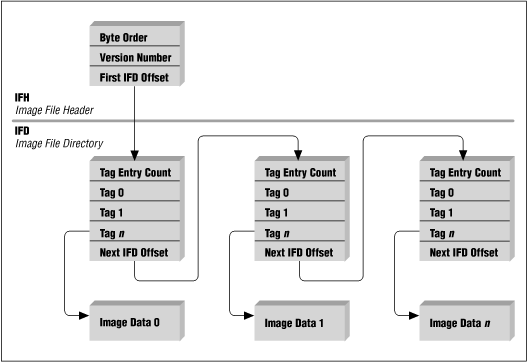
\includegraphics[width=10cm]{./img/tiffFormat.png}
  \caption{TIFF File Structure\cite{Murray1996}}
  \label{fig:tiffFormat}
\end{figure}

For the purposes of this research, only uncompressed TIFF images are used in order to eliminate the need for resource intensive decompression and compression of input and output images.  To support the reading and writing of these image files, the LibTiff libary is cross-compiled for use on the ZC702's PetaLinux OS. 

\subsection{Cross-Compilation}

\subsection{User Interface}

\section{Processor Based Processing}

\section{Programmable Logic Based Processing}

\section{Homogeneous Processing}

